%%This is a very basic article template.
%%There is just one section and two subsections.
\documentclass{article}

\usepackage{graphicx}
\usepackage{underscore}
\usepackage{soul}
\usepackage[colorlinks]{hyperref}
\usepackage{textcomp}
\usepackage{listings}
\usepackage{color}
\usepackage{longtable}

\definecolor{codegreen}{rgb}{0,0.6,0}
\definecolor{codegray}{rgb}{0.5,0.5,0.5}
\definecolor{codepurple}{rgb}{0.58,0,0.82}
\definecolor{backcolour}{rgb}{0.95,0.95,0.82}
 
\lstdefinestyle{mystyle}{
    backgroundcolor=\color{backcolour},   
    commentstyle=\color{codegreen},
    keywordstyle=\color{magenta},
    numberstyle=\tiny\color{codegray},
    stringstyle=\color{codepurple},
    basicstyle=\footnotesize,
    breakatwhitespace=false,         
    breaklines=true,                 
    captionpos=b,                    
    keepspaces=true,                 
    numbers=left,                    
    numbersep=5pt,                  
    showspaces=false,                
    showstringspaces=false,
    showtabs=false,                  
    tabsize=2
}
 
\lstset{style=mystyle}

\begin{document}

\begin{titlepage}

    \centering
    \vfill
    	
\includegraphics{xrootd-logo.png}
    \vfill
    	{\huge \textbf{XRootD Client Configuration \& API Reference} \\}
        \vskip3cm
        \today \\
        Release 4.9.0 and above \\
%        \vskip0.2cm
        Michal Simon (CERN) \\
        \vskip0.2cm
        
\includegraphics[width=3cm, height=3cm]{cern-logo.png}
    \vfill
    \vfill

\end{titlepage}

\tableofcontents

\newpage

\section{Introduction}
    TODO philosophy: \\
    	- connection handling hidden from user \\
    	- 100\% async + event loop \\
    	- threading model: all callbacks in thread-pool + poller thread + timers \\ 
    	- tuned through envvars or XrdCl::DefaultEnv \\
    	- OOD API (doxygen) \\
    	- Posix API (link xrootd.org) \\
    	- New declarative API (ref last section) \\
    	- command line tools (ref xrdcp / xrdfs)
    	
	\ldots\ldots\ldots
	

\section{Configuration File}

	This section describes the XRootD client configuration file. By default XRootD client will use
	the global config file: \textit{/ets/xrootd/client.conf}. However, those settings migh be overwritten
	by the user specific config file: \textit{$\sim$/.xrootd/client.conf} and Environment Variables. For 
	the complete list of configurable parameters please consult the \hyperref[sec:envar]	
	{Index of Environment Variables}. \\
	XRootD client supports protocol- and endpoint-level plug-ins. By convention a single config file is 
	expected per plug-in, as they are discovered and configured by scanning configuration files. The
	plug-in manager will search for configuration files in:
	\begin{itemize}
	  \item /etc/xrootd/client.plugins.d/,
	  \item $\sim$/.xrootd/client.plugins.d/,
	  \item and at a location pointed to by: \hyperref[env:pluginconfigdir]{XRD_PLUGINCONFDIR}
	\end{itemize}
	An XRootD client plug-in configuration file should a contain following key-value pairs:
	\begin{itemize}
	  \item \textbf{url} followed by list of endpoints (by default root protocol is assumed) or protocols
	  \item \textbf{lib} followed by a path to the library implementing given plug-in
	  \item \textbf{enable} followed by \textit{true} or \textit{false} 
	\end{itemize}
	For example the following config file defines a plug-in for \textit{host.domain.edu} endpoint (root 
	protocol is being assumed) and \textit{http} protocol:
	
	\begin{lstlisting}
		url = host.domain.edu;http://*
		lib = /usr/lib64/libAwsomePlugIn.so
		enabled = true
	\end{lstlisting}


\section{Command line tools (xrdcp/xrdfs)}

    \subsection{xrdcp - copy files}
    
		\textbf{xrdcp} [options] source destination \\
		
		\noindent \textbf{DESCRIPTION} \\
		
		\noindent  The \textbf{xrdcp} utility copies one or more files from one location to
		another. The data source and destination may be a local or remote file or directory.
		Additionally, the data source may also reside on multiple servers. \\
		
		\noindent \textbf{OPTIONS} \\
		
		\noindent \textbf{-C} $\vert$ \textbf{\texttt{-{}-}cksum} \underline{type} [\textbf{:}\underline{value} $\vert$ \underline{print} $\vert$ \underline{source}]
		
		\noindent Obtains the checksum of \underline{type} (i.e. adler32, crc32, or md5) from the source,
		computes the checksum at the destination, and verifies that they are the same. If a \underline{value}
		is specified, it is used as the source checksum. When \underline{print} is specified, the checksum at 
		the destination is printed but is \underline{not} verified. \\
		
		\noindent \textbf{-d} $\vert$ \textbf{\texttt{-{}-}debug} \underline{lvl}
		
		\noindent Debug level: 1 (low), 2 (medium), 3 (high). \\
		
		\noindent \textbf{-F} $\vert$ \textbf{\texttt{-{}-}coerce}

		\noindent Ignores locking semantics on the destination file. This option may lead to
		file corruption if not properly used. \\
		
		\noindent \textbf{-f} $\vert$ \textbf{\texttt{-{}-}force}

		\noindent Re-creates a file if it is already present. \\
		
		\noindent \textbf{-h} $\vert$ \textbf{\texttt{-{}-}help}

		\noindent Displays usage information. \\
		
		\noindent \textbf{-H} $\vert$ \textbf{\texttt{-{}-}license}

		\noindent Displays license terms and conditions. \\
		
		\noindent \textbf{-N} $\vert$ \textbf{\texttt{-{}-}nopbar}

		\noindent Does not display the progress bar. \\
		
		\noindent \textbf{-P} $\vert$ \textbf{\texttt{-{}-}posc}

		\noindent Requests POSC (persist-on-successful-close) processing
		to create a new file. Files are automatically deleted should they not be
		successfully closed. \\
		
		\noindent \textbf{-D} $\vert$ \textbf{\texttt{-{}-}proxy} \underline{proxyaddr}\textbf{:}\underline{proxyport} [NOT YET IMPLEMENTED]
		
		\noindent Use \underline{proxyaddr}\textbf{:}\underline{proxyport} as a SOCKS4 proxy. Only numerical addresses are supported. \\

		\noindent \textbf{-r} $\vert$ \textbf{\texttt{-{}-}recursive}

		\noindent Recursively copy all files starting at the given source directory. \\
		
		\noindent \textbf{\texttt{-{}-}server}

		\noindent Runs as if in a server environment. Used only for server-side
		third party copy support. \\
		
		\noindent\textbf{-s} $\vert$ \textbf{\texttt{-{}-}silent}

		\noindent Neither produces summary information nor displays the progress bar. \\
		
		\noindent \textbf{-y} $\vert$ \textbf{\texttt{-{}-}sources} \underline{num}

		\noindent Uses up to \underline{num} sources to copy the file. \\
		
		\noindent \textbf{-S} $\vert$ \textbf{\texttt{-{}-}streams} \underline{num}

		\noindent Uses \underline{num} additional parallel streams to do the transfer.
		The maximum value is 15. The default is 0 (i.e., use only the main stream). \\
		
		\noindent \textbf{\texttt{-{}-}tpc} [\textbf{delegate}] \textbf{first} $\vert$ \textbf{only}

		\noindent Copies the file from remote server to remote server using third-party-copy
		protocol (i.e., data flows from server to server). The source and destination
		servers must support third party copies. Additional security restrictions
		may apply and may cause the copy to fail if they cannot be satisfied.
		Argument '\textbf{first}' tries tpc and if it fails, does a normal copy;
		while '\textbf{only}' fails the copy unless tpc succeeds. When '\textbf{delegate}' is
		specified, the copy delegates the command issuer's credentials to the target
		server which uses those credentials to authenticate with the source server.
		Delegation is ignored if the target server is not configured to use delegated
		credentials. Currently, only gsi credentials can be delegated. \\
		
		\noindent \textbf{-v} $\vert$ \textbf{\texttt{-{}-}verbose}

		\noindent Displays summary output. \\
		
		\noindent \textbf{-V} $\vert$ \textbf{\texttt{-{}-}version}

		\noindent Displays version information and immediately exits. \\
		
		\noindent \textbf{-z} $\vert$ \textbf{\texttt{-{}-}zip} \underline{file}

		\noindent Copy given file from a ZIP archive (same as xrdcl.unzip opaque info). \\
		
		\noindent \textbf{-X} $\vert$ \textbf{\texttt{-{}-}xrate} \underline{rate} [NOT YET IMPLEMENTED]
		
		\noindent Limits the copy speed to the specified \underline{rate}. The rate may be qualified
		with the letter \textbf{k}, \textbf{m}, or \textbf{g} to indicate kilo, mega, or giga
		bytes, respectively. The option only applies when the source or destination is
		local. \\
		
		\noindent \textbf{-Z} $\vert$ \textbf{\texttt{-{}-}dynamic-src}

		\noindent File size may change during the copy. \\
		
		\noindent \textbf{-I} $\vert$ \textbf{\texttt{-{}-}infiles} \underline{fn}

		\noindent Specifies the file that contains a list of input files. \\
		
		\noindent \textbf{-p} $\vert$ \textbf{\texttt{-{}-}path}

		\noindent Automatically create remote destination path. \\
		
		\noindent \textbf{\texttt{-{}-}parallel} \underline{n}

		\noindent Number of copy jobs to be run simultaneously. \\
		
		\noindent \textbf{\texttt{-{}-}allow-http}

		\noindent Allow HTTP as source or destination protocol. Requires the XrdClHttp client plugin. \\
		
		\noindent \textbf{LEGACY OPTIONS} \\
		
		\noindent Legacy options are provided for backward compatability. These are now
		deprecated and should be avoided. \\
		
		\noindent \textbf{-adler}

		\noindent Equivalent to "\textbf{--cksum adler32:source}". \\
		
		\noindent \textbf{-DI} \underline{pname} \underline{numberval}

		\noindent Set the internal parameter \underline{pname} with the numeric value \underline{numberval}. \\
		
		\noindent \textbf{-DS} \underline{pname} \underline{stringval}

		\noindent Set the internal parameter \underline{pname} with the string value \underline{stringval}. \\
		
		\noindent \textbf{-md5}

		\noindent Equivalent to "\textbf{--cksum md5:source}". \\
		
		\noindent \textbf{-np}

		\noindent Equivalent to "\textbf{--nopbar}". \\
		
		\noindent \textbf{-OD} \underline{cgi}

		\noindent Add cgi information \underline{cgi} to any destination xrootd URL.
		You should specify the opaque information directly on the destination URL. \\
		
		\noindent \textbf{-OS} \underline{cgi}

		\noindent Add cgi information \underline{cgi} to any source xrootd URL. \\
		
		\noindent \textbf{-x}

		\noindent Equivalent to "\textbf{--sources 12}". \\
		
		\pagebreak
		\noindent \textbf{OPERANDS} \\
		
		\noindent \underline{source}: a dash (i.e. \textbf{-}) indicating stanard in, a local file, a local directory 
		name suffixed by /, or an xrootd URL in the form of:
		
		\textbf{xroot://} [\underline{user}\textbf{@}] \underline{host} [\textbf{:}\underline{port}] /absolutepath
		
		\noindent The \underline{absolutepath} can be a directory. \\
		
		\noindent \underline{destination}: a dash (i.e. \textbf{-}) indicating stanard out, a local file, a local directory
		name suffixed by /, or an xrootd URL in the form:

		\textbf{xroot://} [\underline{user}\textbf{@}] \underline{host} [\textbf{:}\underline{port}] /absolutepath

		\noindent The \underline{absolutepath} can be a directory. \\
		
    \subsection{xrdfs - xrootd file and directory meta-data utility}
    	\ldots\ldots\ldots

	\subsection{Return Codes}
		\begin{itemize}
  			\item \textbf{50} : generic error (e.g. config, internal, data, OS, command line option)
  			\item \textbf{51} : socket related error
			\item \textbf{52} : postmaster related error
			\item \textbf{53} : XRootD related error
			\item \textbf{54} : redirection error
			\item \textbf{55} : query response was negative (this is not an error)
		\end{itemize}



\section{Environment Variables}

	This section describes XRootD client environment variables. The following list of environment 
	variables applies to \textit{xrdcp}, \textit{xrdfs} any other application using the libXrdCl 
	library, unless specified otherwise.
	
	\subsection{Categories}
		\begin{center}
		  \begin{longtable}{ | l | p{0.5\textwidth} | }
		    \hline
		    {\footnotesize \textbf{Limits/Performance:}} & \begin{scriptsize}
		    \begin{itemize}
		      \item \hyperref[env:parallelevtloop]{XRD_PARALLELEVTLOOP}
		      \item \hyperref[env:redirectlimit]{XRD_REDIRECTLIMIT}
		      \item \hyperref[env:substreamsperchannel]{XRD_SUBSTREAMSPERCHANNEL}
		      \item \hyperref[env:workerthreads]{XRD_WORKERTHREADS}
	   	    \end{itemize} 
		  	\end{scriptsize} \\
		    \hline
		    
		     {\footnotesize \textbf{Logging:}} & \begin{scriptsize} 
		     \begin{itemize}
	     	   \item \hyperref[env:loglevel]{XRD_LOGLEVEL}
	     	   \item \hyperref[env:logfile]{XRD_LOGFILE}
	     	   \item \hyperref[env:logmask]{XRD_LOGMASK}
		     \end{itemize} 
			 \end{scriptsize} \\ 
		     \hline
		     
		     {\footnotesize \textbf{Metalinks:}} & \begin{scriptsize}
		     \begin{itemize}
		       \item \hyperref[env:metalinkprocessing]{XRD_METALINKPROCESSING}
      	       \item \hyperref[env:localmetalinkfile]{XRD_LOCALMETALINKFILE}
		       \item \hyperref[env:glfnredirector]{XRD_GLFNREDIRECTOR}
		       \item \hyperref[env:maxmetalinkwait]{XRD_MAXMETALINKWAIT}
		     \end{itemize} 
		     \end{scriptsize} \\ 
		     \hline
		     
		     {\footnotesize \textbf{Monitoring:}} & \begin{scriptsize} 
		     \begin{itemize}
		       \item \hyperref[env:appname]{XRD_APPNAME}
		       \item \hyperref[env:clientmonitor]{XRD_CLIENTMONITOR}
		       \item \hyperref[env:clientmonitorparam]{XRD_CLIENTMONITORPARAM}
		     \end{itemize}
		     \end{scriptsize} \\
		     \hline
		     
		     {\footnotesize \textbf{Networking:}} & \begin{scriptsize} 
		     \begin{itemize}
		       \item \hyperref[env:networkstack]{XRD_NETWORKSTACK}
		       \item \hyperref[env:preferipv4]{XRD_PREFERIPV4}
		     \end{itemize} 
		     \end{scriptsize} \\
		     \hline
		     
		     {\footnotesize \textbf{Plug-in:}} & \begin{scriptsize}
		     \begin{itemize}
		       \item \hyperref[env:plugin]{XRD_PLUGIN}
		       \item \hyperref[env:pluginconfigdir]{XRD_PLUGINCONFDIR}
		     \end{itemize} 
		     \end{scriptsize} \\
		     \hline
		     
		     {\footnotesize \textbf{Recovery:}} & \begin{scriptsize} 
		     \begin{itemize}
		       \item \hyperref[env:connectionretry]{XRD_CONNECTIONRETRY}
		       \item \hyperref[env:openrecovery]{XRD_OPENRECOVERY}
		       \item \hyperref[env:readrecovery]{XRD_READRECOVERY}
		       \item \hyperref[env:writerecovery]{XRD_WRITERECOVERY}
		       \item \hyperref[env:streamerrorwindow]{XRD_STREAMERRORWINDOW}
		     \end{itemize} 
		     \end{scriptsize} \\
		     \hline
		     
		     {\footnotesize \textbf{TCP:}} & \begin{scriptsize} 
		     \begin{itemize}
		       \item \hyperref[env:nodelay]{XRD_NODELAY}
		       \item \hyperref[env:tcpkeepalive]{XRD_TCPKEEPALIVE}
		       \item \hyperref[env:tcpkeepaliveinterval]{XRD_TCPKEEPALIVEINTERVAL}
		       \item \hyperref[env:tcpkeepaliveprobes]{XRD_TCPKEEPALIVEPROBES}
		       \item \hyperref[env:tcpkeepalivetime]{XRD_TCPKEEPALIVETIME}
		     \end{itemize} 
		     \end{scriptsize} \\ 
		     \hline
		     
		     {\footnotesize \textbf{Timeouts:}} & \begin{scriptsize} 
		     \begin{itemize}
		       \item \hyperref[env:connectionwindow]{XRD_CONNECTIONWINDOW}
		       \item \hyperref[env:requesttimeout]{XRD_REQUESTTIMEOUT}
		       \item \hyperref[env:streamtimeout]{XRD_STREAMTIMEOUT}
		       \item \hyperref[env:dataserverttl]{XRD_DATASERVERTTL}
		       \item \hyperref[env:loadbalancerttl]{XRD_LOADBALANCERTTL}
		       \item \hyperref[env:timeoutresolution]{XRD_TIMEOUTRESOLUTION}
		     \end{itemize} 
		     \end{scriptsize} \\ 
		     \hline
		     
		     {\footnotesize \textbf{XrCl::CopyProcess / xrdcp:}} & \begin{scriptsize} 
		     \begin{itemize}
		       \item \hyperref[env:cpchunksize]{XRD_CPCHUNKSIZE}
		       \item \hyperref[env:cpinittimeout]{XRD_CPINITTIMEOUT}
		       \item \hyperref[env:cptpctimeout]{XRD_CPTPCTIMEOUT}
		       \item \hyperref[env:cpparallelchunks]{XRD_CPPARALLELCHUNKS}
		       \item \hyperref[env:xcpblocksize]{XRD_XCPBLOCKSIZE}
		     \end{itemize} 
		     \end{scriptsize} \\
		     \hline
		     
		     {\footnotesize \textbf{Others:}} & \begin{scriptsize} 
		     \begin{itemize}
		       \item \hyperref[env:pollerpreference]{XRD_POLLERPREFERENCE}
		       \item \hyperref[env:runforkhandler]{XRD_RUNFORKHANDLER}
		     \end{itemize} 
		     \end{scriptsize} \\
		     \hline
		     
		  \end{longtable}
		\end{center}

	\subsection{Index of Environment Variables}
	\label{sec:envar}
	
		\subsubsection{XRD_APPNAME}
		\label{env:appname}
		    Override the application name reported to the server. \\
		    \textbf{Default: disabled}
		    
		\subsubsection{XRD_CLIENTMONITOR}
		\label{env:clientmonitor}
		    Path to the client monitor library. \\
		    \textbf{Default: disabled}
		
		\subsubsection{XRD_CLIENTMONITORPARAM}
		\label{env:clientmonitorparam}
		    Additional optional parameters that will be passed to the monitoring object on initialization. \\
		    \textbf{Default: disabled}
		    
		\subsubsection{XRD_CONNECTIONWINDOW}
		\label{env:connectionwindow}
			A time window for the connection establishment. A connection failure is declared if the connection is not 
			established within the time window. If a connection failure happens earlier then another connection attempt 
			will only be made at the beginning of the next window. \\
			\textbf{Default: 120} (seconds)
		
		\subsubsection{XRD_CONNECTIONRETRY}
		\label{env:connectionretry}
		    Number of connection attempts that should be made (number of available connection windows) before declaring 
		    a permanent failure. \\
		    \textbf{Default: 5}
		
		\subsubsection{XRD_CPCHUNKSIZE}
		\label{env:cpchunksize}
		    Size of a single data chunk handled by xrdcp / XrdCl::CopyProcess. \\
		    \textbf{Default: 16KiB}
		    		
		\subsubsection{XRD_CPINITTIMEOUT}
		\label{env:cpinittimeout}
		    Maximum time allowed for the copy process to initialize, ie. open the source and destination files. \\
		    \textbf{Default: 600} (seconds)
		    
		\subsubsection{XRD_CPPARALLELCHUNKS}
		\label{env:cpparallelchunks}
		    Maximum number of asynchronous requests being processed by the xrdcp / XrdCl::CopyProcess command at any given 
		    time. \\
		    \textbf{Default: 4}
		    
		\subsubsection{XRD_CPTPCTIMEOUT}
		\label{env:cptpctimeout}
		    Maximum time allowed for a third-party copy operation to finish. \\
		    \textbf{Default: 1800} (seconds)
		    
		\subsubsection{XRD_DATASERVERTTL}
		\label{env:dataserverttl}
		    Time period after which an idle connection to a data server should
		    be closed. \\
		    \textbf{Default: 300} (seconds)
		    
		\subsubsection{XRD_GLFNREDIRECTOR}
		\label{env:glfnredirector}
		    The redirector will be used as a last resort if the GLFN tag is specified in a Metalink file. \\
		    \textbf{Default: none}
		    
		\subsubsection{XRD_LOADBALANCERTTL}
		\label{env:loadbalancerttl}
			Time period after which an idle connection to a manager or a load balancer should be closed. \\
			\textbf{Default: 1200} (seconds)
			
		\subsubsection{XRD_LOCALMETALINKFILE}
		\label{env:localmetalinkfile}
		    Enable/Disable local Metalink file processing (by convention the following URL schema has to be used: 
		    \textit{root://localfile//path/filename.meta4}) The \textit{localfile} semantic is now deprecated, use 
		    \textit{file://localhost/path/filename.meta4} instead! \\
		    \textbf{Default: 0}
		    
		\subsubsection{XRD_LOGFILE}
		\label{env:logfile}
			If set, the diagnostics will be printed to the specified file instead of \textit{stderr}. \\
			\textbf{Default: disabled}
			
		\subsubsection{XRD_LOGLEVEL}
		\label{env:loglevel}
			Determines the amount of diagnostics that should be printed. Valid values are: \ul{Dump}, 
			\ul{Debug}, \ul{Info}, \ul{Warning}, and \ul{Error}. \\
     	    \textbf{Default: disabled}
			
		\subsubsection{XRD_LOGMASK}
		\label{env:logmask}
		
			Determines which diagnostics topics should be printed at all levels. It's a "$\vert$" separated list of 
			topics. The first element may be ``All" in which case all the topics are enabled and the subsequent
			elements may turn them off, or "None" in which case all the topics are disabled and the subsequent 
		 	flags may turn them on. If the topic name is prefixed with "\textasciicircum", then it means that the 
		 	topic should be disabled. If the topic name is not prefixed, then it means that the topic should be enabled.
			
		 	The log mask may as well be handled for each diagnostic level separately by setting one or more of 
		 	the following variables: \ul{XRD_LOGMASK_ERROR}, \ul{XRD_LOGMASK_WARNING}, 
		 	\ul{XRD_LOGMASK_INFO}, \ul{XRD_LOGMASK_DEBUG}, and \ul{XRD_LOGMASK_DUMP}. 
		 				
		 	Available topics: AppMsg, UtilityMsg, FileMsg, PollerMsg, PostMasterMsg, XRootDTransportMsg, TaskMgrMsg, 
		 	XRootDMsg, FileSystemMsg, AsyncSock\-Msg \\
		 	\textbf{Default:} The default for each level is	\textbf{"All"}, except for the \ul{Dump} level, where the default 
		 	is \textbf{"All$\vert$ \textasciicircum PollerMsg"}. This means that, at the \ul{Dump} level, all the topics but 
		 	"PollerMsg" are enabled.
		 	
		 	
		\subsubsection{XRD_MAXMETALINKWAIT}
		\label{env:maxmetalinkwait}
		    The maximum time in seconds a client can be stalled by the server if a Metalink redirector is available. \\
		    \textbf{Default: 60} (seconds)
		    
		\subsubsection{XRD_METALINKPROCESSING}
		\label{env:metalinkprocessing}
		    Enable/Disable Metalink processing. \\
		    \textbf{Default: 1}
		    
		\subsubsection{XRD_NETWORKSTACK}
		\label{env:networkstack}
		    The network stack that the client should use to connect to the server. Possible values are:
			\begin{itemize}
		    \item \textbf{IPAuto} - automatically detect which IP stack to use 
		    \item \textbf{IPAll} - use IPv6 stack (AF_INET6 sockets) and both IPv6 and IPv4 (mapped to IPv6) addresses
		    \item \textbf{IPv6} - use only IPv6 stack and addresses
		    \item \textbf{IPv4} - use only IPv4 stack (AF_INET sockets) and addresses
		    \item \textbf{IPv4Mapped6} - use IPv6 stack and mapped IPv4 addresses
		    \end{itemize}
		    \textbf{Default: IPAuto}
		    
		\subsubsection{XRD_NODELAY}
		\label{env:nodelay}
		    Disables the Nagle algorithm if set to 1 (default), enables it if set to 0. \\
		    \textbf{Default: 1}
		    
		\subsubsection{XRD_OPENRECOVERY}
		\label{env:openrecovery}
			Determines if open recovery should be enabled or disabled for mutable (truncate or create) opens. \\
			\textbf{Default: true}
			
		\subsubsection{XRD_PARALLELEVTLOOP}
		\label{env:parallelevtloop}
			The number of event loops. \\
			\textbf{Default: 1}

		\subsubsection{XRD_PLUGIN}
		\label{env:plugin}
			A default client plug-in to be used. \\
			\textbf{Default: none}

		\subsubsection{XRD_PLUGINCONFDIR}
		\label{env:pluginconfigdir}
		    A custom location containing client plug-in config files. \\
		    \textbf{Default: none}
		    
		\subsubsection{XRD_POLLERPREFERENCE}
		\label{env:pollerpreference}
		    A comma separated list of poller implementations in order of preference. \\
		    \textbf{Default: built-in}

		\subsubsection{XRD_PREFERIPV4}
		\label{env:preferipv4}
		    If set the client tries first IPv4 address (turned off by default). \\
		    \textbf{Default: 0}
		    
		\subsubsection{XRD_READRECOVERY}
		\label{env:readrecovery}
		    Determines if read recovery should be enabled or disabled. \\
		    \textbf{Default: true}
		
		\subsubsection{XRD_REDIRECTLIMIT}
		\label{env:redirectlimit}
		    Maximum number of allowed redirections. \\
		    \textbf{Default: 16}
		    
		\subsubsection{XRD_REQUESTTIMEOUT}
		\label{env:requesttimeout}
		    Default value for the time after which an error is declared if it was impossible to get a response to a 
		    request. \\
		    \textbf{Default: 1800} (seconds)
		    
		\subsubsection{XRD_RUNFORKHANDLER}
		\label{env:runforkhandler}
		    Determines whether the fork handlers should be enabled, making the API fork safe. \\
		    \textbf{Default: 0}
		    
		\subsubsection{XRD_STREAMERRORWINDOW}
		\label{env:streamerrorwindow}
		    Time after which the permanent failure flags are cleared out and a new connection may be attempted if needed. \\
		    \textbf{Default: 1800}
		    
		\subsubsection{XRD_STREAMTIMEOUT}
		\label{env:streamtimeout}
		    Default value for the time after which a connection error is declared (and a recovery attempted) if there are 
		    unfulfilled requests and there is no socket activity or a registered wait timeout. \\
		    \textbf{Default: 60} (seconds)
		    
		\subsubsection{XRD_SUBSTREAMSPERCHANNEL}
		\label{env:substreamsperchannel}
			Number of streams per session. \\
			\textbf{Default: 1}
			
		\subsubsection{XRD_TCPKEEPALIVE}
		\label{env:tcpkeepalive}
		    Enable/Disable the TCP keep alive functionality. \\
		    \textbf{Default: 0}
		    
		\subsubsection{XRD_TCPKEEPALIVEINTERVAL}
		\label{env:tcpkeepaliveinterval}
		    Interval between subsequent keepalive probes (Linux only). \\
		    \textbf{Default: 75}
		    
		\subsubsection{XRD_TCPKEEPALIVEPROBES}
		\label{env:tcpkeepaliveprobes}
		    Number of unacknowledged probes before considering the connection dead (Linux only). \\
		    \textbf{Default: 9}
		    
		\subsubsection{XRD_TCPKEEPALIVETIME}
		\label{env:tcpkeepalivetime}
		    Time between last data packet sent and the first keepalive probe (Linux only). \\
		    \textbf{Default: 7200}
		    
		\subsubsection{XRD_TIMEOUTRESOLUTION}
		\label{env:timeoutresolution}
		    Resolution for the timeout events. Ie. timeout events will be processed only every XRD_TIMEOUTRESOLUTION 
		    seconds. \\
		    \textbf{Default: 15} (seconds)
		
		\subsubsection{XRD_WORKERTHREADS}
		\label{env:workerthreads}
		    Number of threads processing user callbacks. \\
		    \textbf{Default: 3}
		
		\subsubsection{XRD_WRITERECOVERY}
		\label{env:writerecovery}
			Determines if write recovery should be enabled or disabled. \\
			\textbf{Default: true}

		\subsubsection{XRD_XCPBLOCKSIZE}
		\label{env:xcpblocksize}
		    Maximu size of a data block assigned to a single source in case of an extreme copy transfer. \\
		    \textbf{Default: 128MiB}

    
	\subsection{Timeouts Explained}
		
		\subsubsection{Connection Window and Connection Retry}
			The \hyperref[env:connectionwindow]{\textit{ConnectionWindow}} parameter is applied during client-server connection and 
			controls two aspects of this process:
			\begin{itemize}
			  \item First of all, it controls the length of time allowed to establish an XRootD connection (physical connection, 
	  				XRootD hand-shake, and authentication if required). It is important to note that \textbf{\textit{Connection Window} 
	  				is applied per physical address}. This means that if a connection fails before the end of current 
	  				\textit{ConnectionWindow} and another physical address is available it will be tried immediately.
	  		  \item Secondly (if there are no more available physical addresses), it defines the length of time that must elapse
	  		  		after a connection failure before the connection can be retried. More precisely, the client has to wait until
	  		  		the end of the current \textit{ConnectionWindow} before attempting another connection. The number of retries 
	  		  		that might be attempted is controlled by \hyperref[env:connectionretry]{\textit{ConnectionRetry}} environment 
	  		  		variable.
			\end{itemize} 
			Let us illustrate all this with following example. Suppose XRootD client wants to connect to a server with three
			physical IP address (2x IPv6 and 1x IPv4). For the sake of argument let us suppose it will fail after 60s during the
			hand-shake procedure, while connecting to the $1^{st}$ IPv6 address. What will happen next? Since there are two more
			addresses available, the client will immediately proceed to the next one. Now let us suppose that the cumulative time
			spent on establishing the physical connection and on carrying out the hand-shake exceeded 120s (nominal value of 
			\textit{ConnectionWindow}). In this case the second connection attempt will be timed out, and XRootD client will proceed
			to the $3^{rd}$ IP address. Again, let us suppose that similarly as in case of the $1^{st}$ IP address the connection
			failed after 60s. Since there are no more address to try, the client will have to wait until the end of the current
			\textit{ConnectionWindow} (that is for another 60s) before the connection procedure can be restarted. Now how all this 
			relates to the \textit{ConnectioRetry}? The nominal value of \textit{ConnectioRetry} is 5, which means we can retry the 
			whole procedure four more times (Note: \textbf{\textit{ConnectionRetry} is not applied per single physical connection 
			but rather to the whole connection procedure}).

		\subsubsection{Stream Timeout}
			The \hyperref[env:streamtimeout]{\textit{StreamTimeout}} parameter is applied during every request/response exchange after 
			the client and the server established a connection. It defines the maximum length of time that may elapse between the moment 
			when the client has sent a request and the moment when the client has received a response for the request in question. If the 
			time spent waiting for response from the server exceeds the \textit{StreamTimeout} an error is declared (and the client will 
			disconnect form the server). \\
			There are two exceptions to the above stated rule:
			\begin{itemize}
			  \item The server may force the client to reissue the request by sending \href{http://xrootd.org/doc/dev49/XRdv400.htm#_Toc517297831}
			  		{\textit{kXR_wait}} response. In this case \textit{StreamTimeout} does not apply to the original request anymore. 
			  \item The server may explicitly instruct the client to not apply the \textit{StreamTimeout} to given request by sending
			  	    \href{http://xrootd.org/doc/dev49/XRdv400.htm#_Toc517297832}{\textit{kXR_waitresp}}.
			\end{itemize} 
		
		\subsubsection{Stream Error Window}
			The \hyperref[env:streamerrorwindow]{\textit{StreamErrorWindow}} controls the length of time that needs to elapse after a 
			fatal error before the client may attempt to reconnect to the server. A fatal error is declared eg. if the host name cannot be 
			resolved, a low level Posix system call fails (eg. \textit{connect}/\textit{fcntl}/\textit{epool}), or client runs out of connection 
			retries. 
		
		\subsubsection{RequestTimeout}
			The \hyperref[env:requesttimeout]{\textit{RequestTimeout}} parameter is applied to a logical XRootD operation (eg. opening a file, 
			listing directory, etc.) as a whole. It is the maximum length of time that may elapse from the moment an operation has been issued 
			using XRootD client API until it has been resolved (no matter how many underlying requests it will trigger). If the \textit{RequestTimeout} 
			is exceeded an error is declared and the operation is resolved as failed. \\ 
			Note: The value of this parameter might be overwritten directly by the user of XRootD client API by setting the timeout argument.
			
		
		\subsubsection{Time To Live}
			A Time To Live (TTL) timeout controls the lifetime of an idle physical connection. If for the given communication channel the time
			length elapsed from last exchange of request/response between the client and server exceeds the TTL timeout the given connection
			will be terminated. There are two types of TTL timeouts in XRootD client:
			\begin{itemize}
			  \item \hyperref[env:dataserverttl]{\textit{DataServerTTL}}: a TTL timeout that is applied to Data Servers
			  \item \hyperref[env:loadbalancerttl]{\textit{LoadBalancerTTL}}: a TTL timeout that is applied to Managers
			\end{itemize}

			
		\subsubsection{How does it all come together?}
			Let us now consider an example in order to illustrate how all those timeouts play along (\textbf{for clarity please consult the diagram 
			below}). Suppose that an \textit{XrdCl::File::Open(\ldots)} operation is being called and that there is no open connection between the 
			client and the server. The client will have to establish the XRootD connection first (subject to \textbf{\textit{ConnectionWindow}}):
			\begin{itemize}
			  \item open physical connection
			  \item carry out hand-shake procedure (\textit{kXR_protocol}, \textit{kXR_login}, etc.)
			\end{itemize}
			Subsequently, the client will issue a \textit{kXR_open} request (subject to \textbf{\textit{StreamTimeout}}). Let us suppose 
			that the server will respond with a \textit{kXR_redirect} redirecting the client to a data server. In this case, the client will 
			have to open another XRootD connection (again, subject to \textbf{\textit{ConnectionWindow}}) and then send an open request
			(again, subject to \textbf{\textit{StreamTimeout}}). Finally, once the server responds, the open operation will be resolved. The whole
			process described in the scenario above is subject to \textbf{\textit{RequestTimeout}}. \\
			Once the connections to the manager and data server become idle they will be subject to respective \textbf{\textit{TTL timeouts}}. \\			
			
			\begin{center}
   				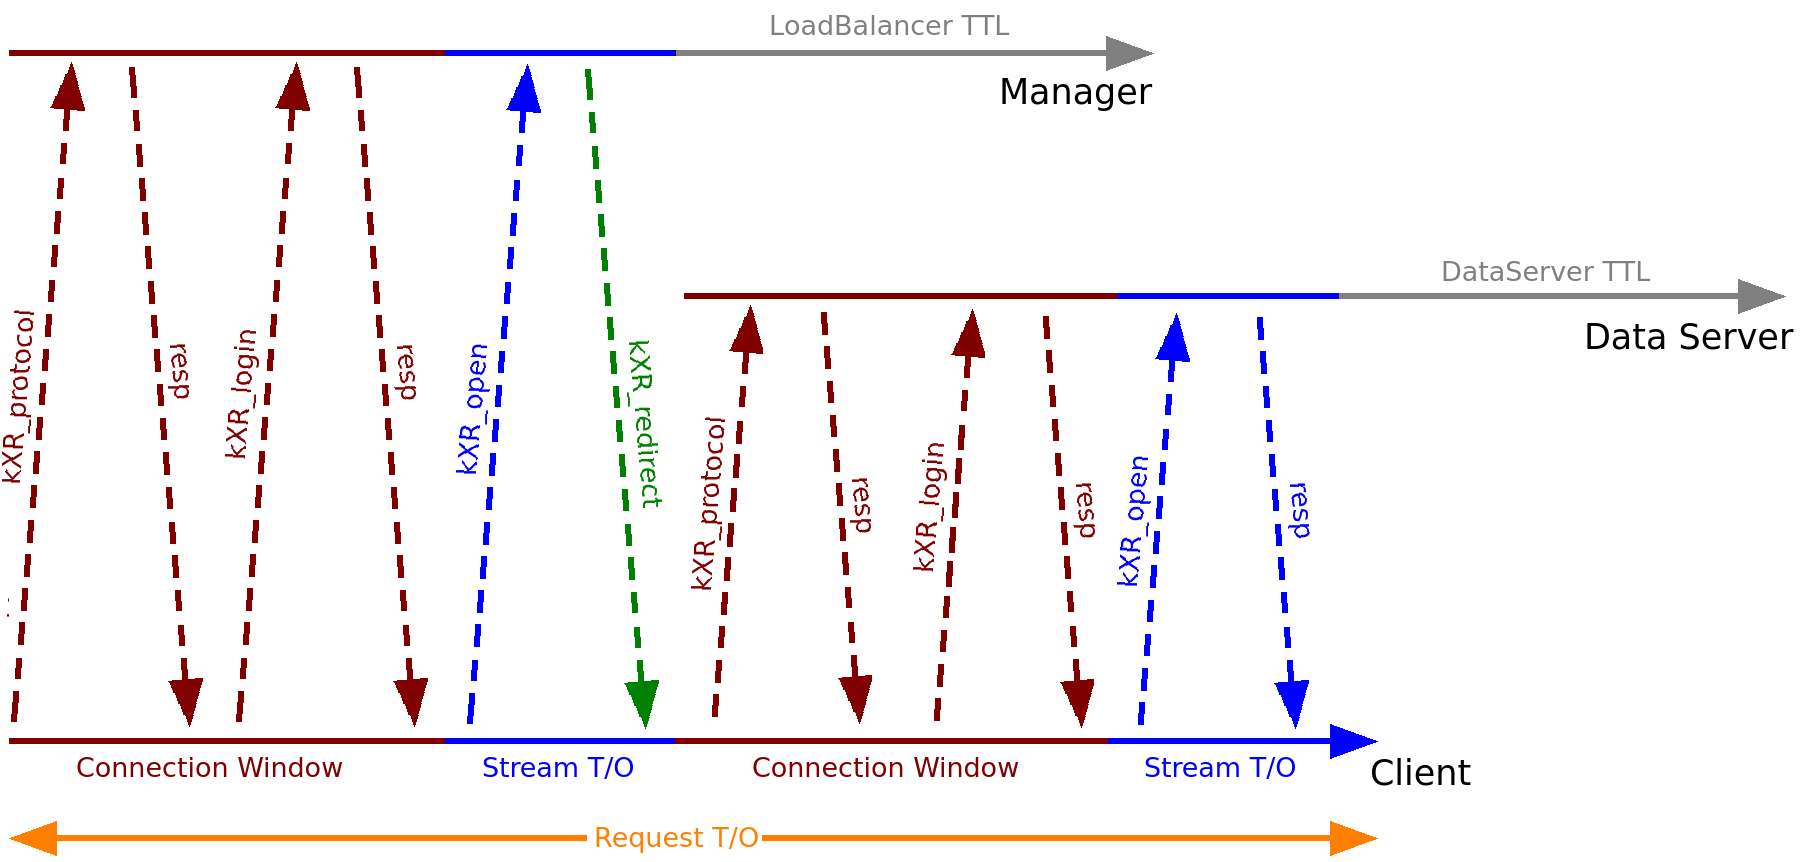
\includegraphics[scale=0.25]{timeout.png}
   			\end{center}

			
		\subsubsection{xrdcp / XrdCl::CopyProcess Third-Party-Copy timeouts}
			The \hyperref[env:cpinittimeout]{\textit{CPInitTimeout}} parameter is applied during initialization of a Third-Party-Copy (TPC) transfer.
			It defines the maximum length of time that may elapse until TPC transfer has been initialized (ie. \textit{open} destination, \textit{open}
			source, issue \textit{sync}, for more details please consult the \href{http://xrootd.org/doc/dev49/tpc_protocol.htm}{TPC Protocol Reference}). \\
			The \hyperref[env:cptpctimeout]{\textit{CPTPCTimeout}} parameter defines the maximum length of time that may elapse between the moment when
			the actual transfer has been started and the moment when it is finished (ie. it is applied to the second \textit{sync}, for more details please 
			consult the \href{http://xrootd.org/doc/dev49/tpc_protocol.htm}{TPC Protocol Reference}). 


\section{Client Declarative API}

	This section describes XRootD client declarative API introduced in 4.9.0. For the standard 
	\textit{XrdCl::File} and \textit{XrdCl::FileSystem}API please consult our \href{http://xrootd.org/doc/doxygen/current/html/annotated.html}
	{Doxygen} documentation. 
	
	\subsection{List of Operations}
	
	open, close, read, write \ldots\ldots\ldots \\
	+
	arguments and response type
	
	\subsection{Special Operations}
	
	parallel, later optional
	
	\subsection{Operation Handlers}
	
	ResponseHandler, function/functor/lambda, std::future, std::packaged_task
	
	\subsection{Utilities}
	
	Fwd class
	
	\subsection{Pipelining Semantics}
	
	examples on how to create and run pipelines
	



\end{document}
